% !TeX root = ba.tex

\section{Appendix}

\begin{figure}
	\centering
	
	\begin{subfigure}{.23\textwidth}
		\centering
		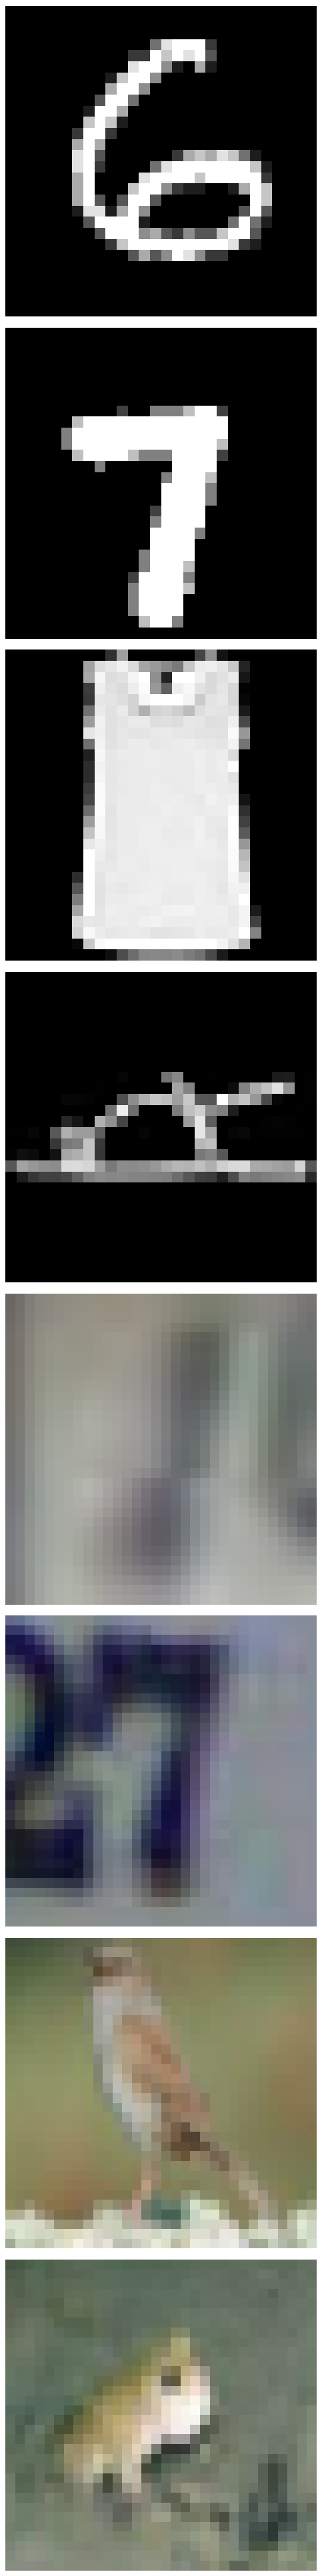
\includegraphics[width=.743478\textwidth, left]{carlini_wagner_orig_appendix.pdf}%
		\caption{Original}%
	\end{subfigure}%
	\begin{subfigure}{.36\textwidth}
		\centering
		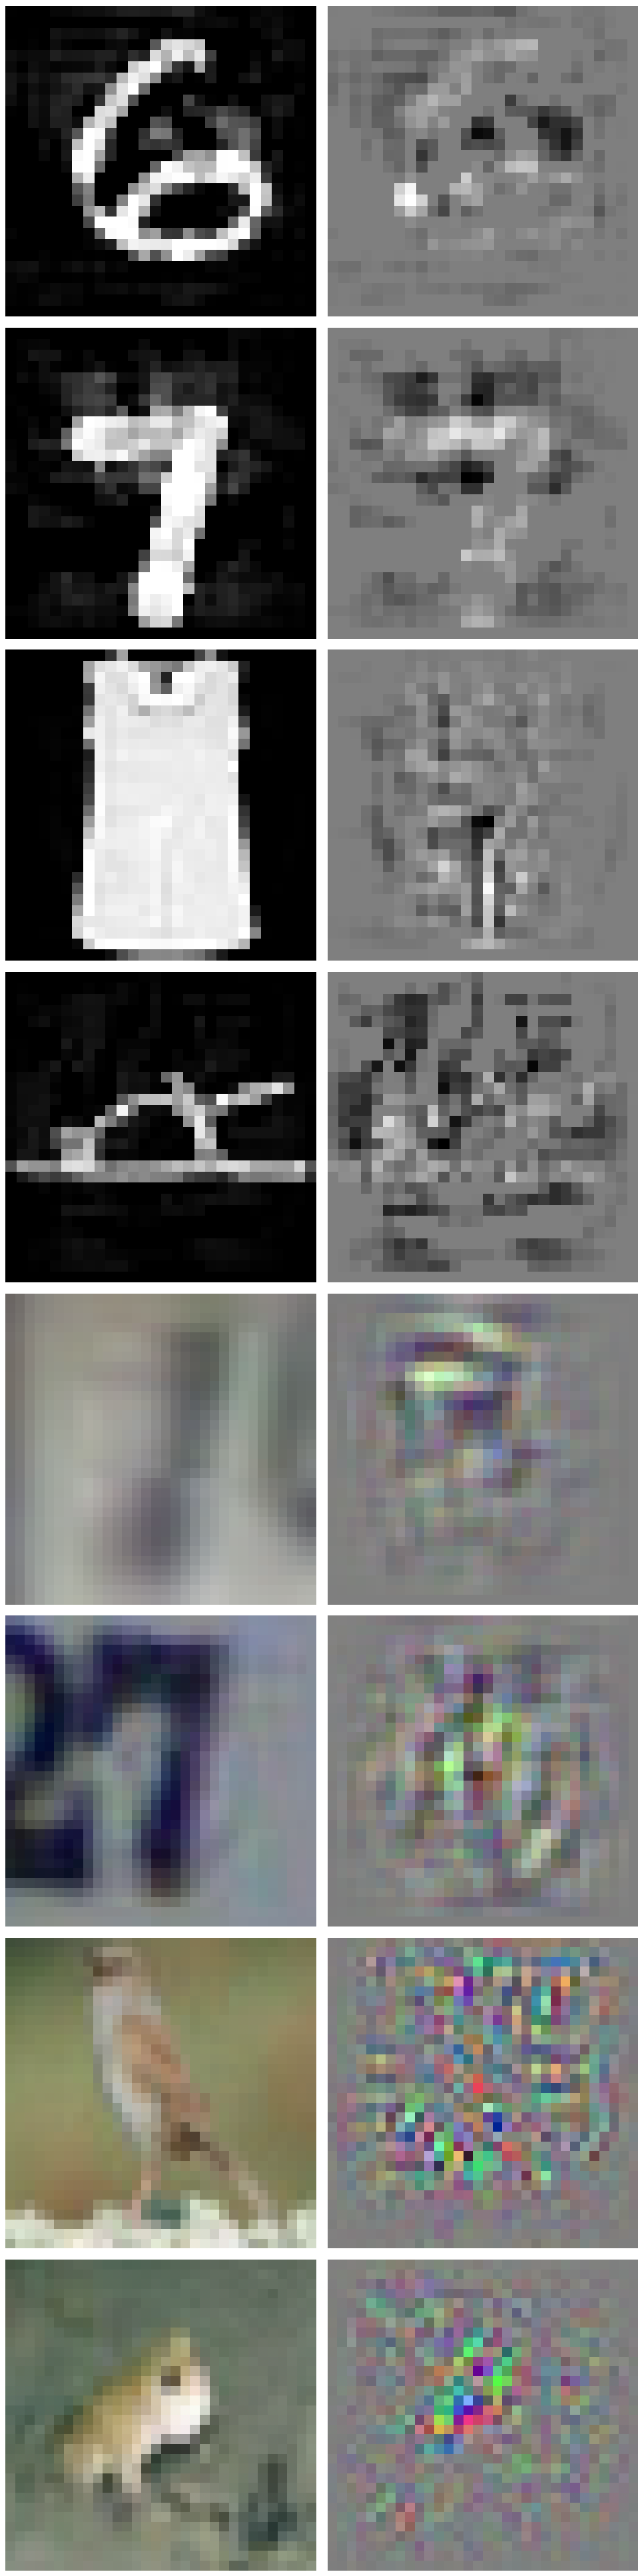
\includegraphics[width=.95\textwidth, center]{carlini_wagner_caps_appendix.pdf}%
		\caption{CapsNet}
	\end{subfigure}%
	\begin{subfigure}{.36\textwidth}
		\centering
		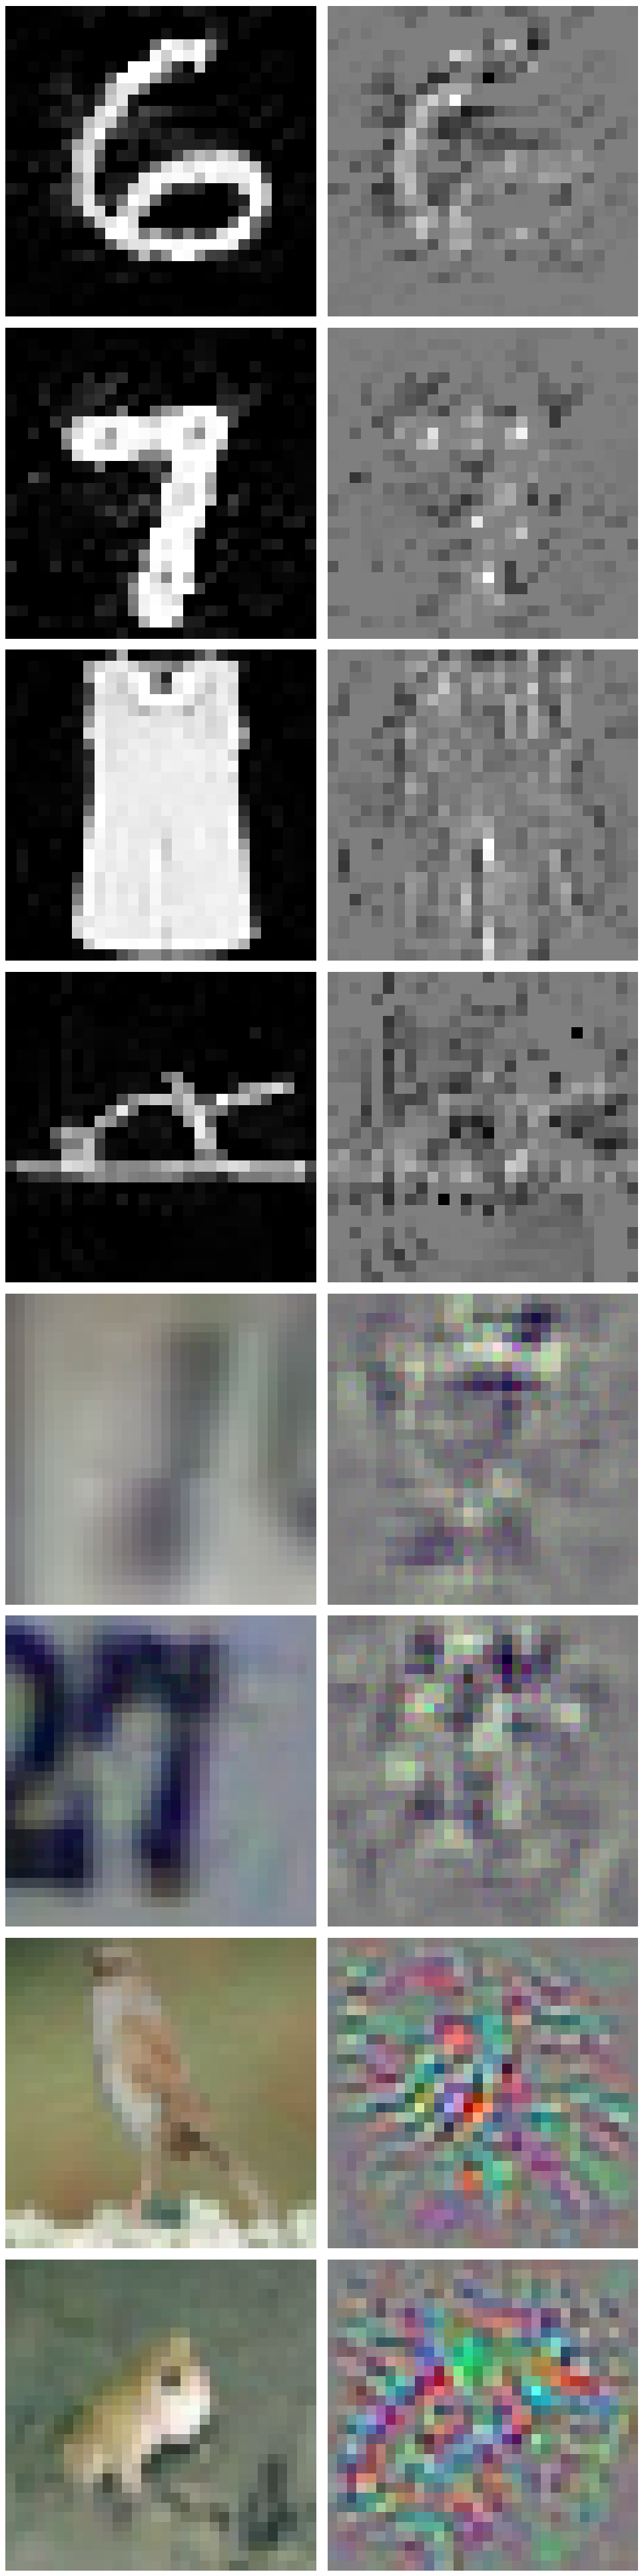
\includegraphics[width=.95\textwidth, right]{carlini_wagner_conv_appendix.pdf}%
		\caption{ConvNet}
	\end{subfigure}
	\caption[Carlini-Wagner Adversarial Examples]{Carlini-Wagner adversarial examples and perturbations. Pixel values of perturbation images are scaled for visibility}
	\label{fig:carlini-wagner-img}
	
\end{figure}


\begin{figure}
	\centering
	
	\begin{subfigure}{.23\textwidth}
		\centering
		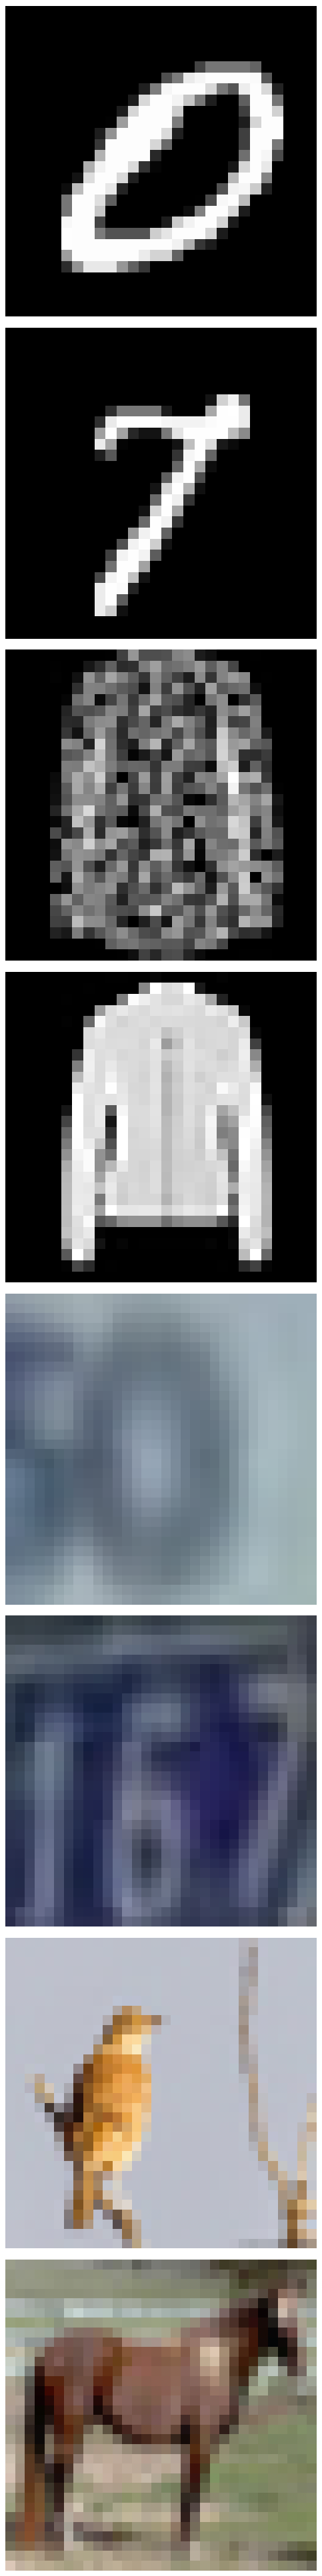
\includegraphics[width=.743478\textwidth, left]{deepfool_orig_appendix.pdf}%
		\caption{Original}%
	\end{subfigure}%
	\begin{subfigure}{.36\textwidth}
		\centering
		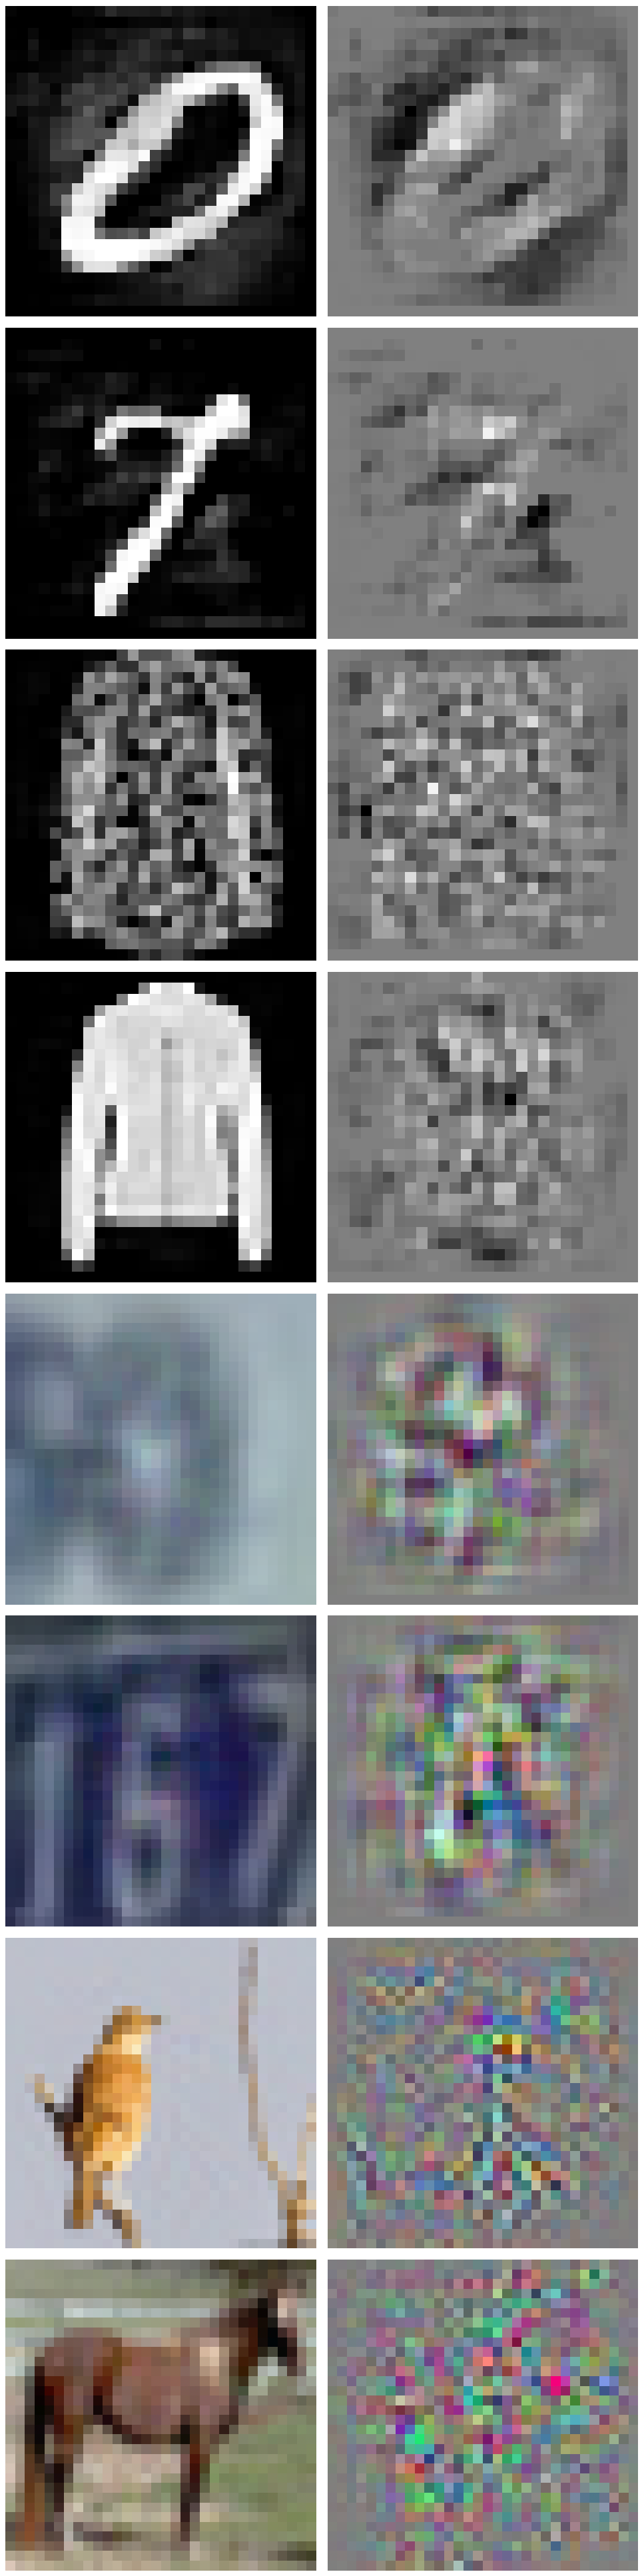
\includegraphics[width=.95\textwidth, center]{deepfool_caps_appendix.pdf}%
		\caption{CapsNet}
	\end{subfigure}%
	\begin{subfigure}{.36\textwidth}
		\centering
		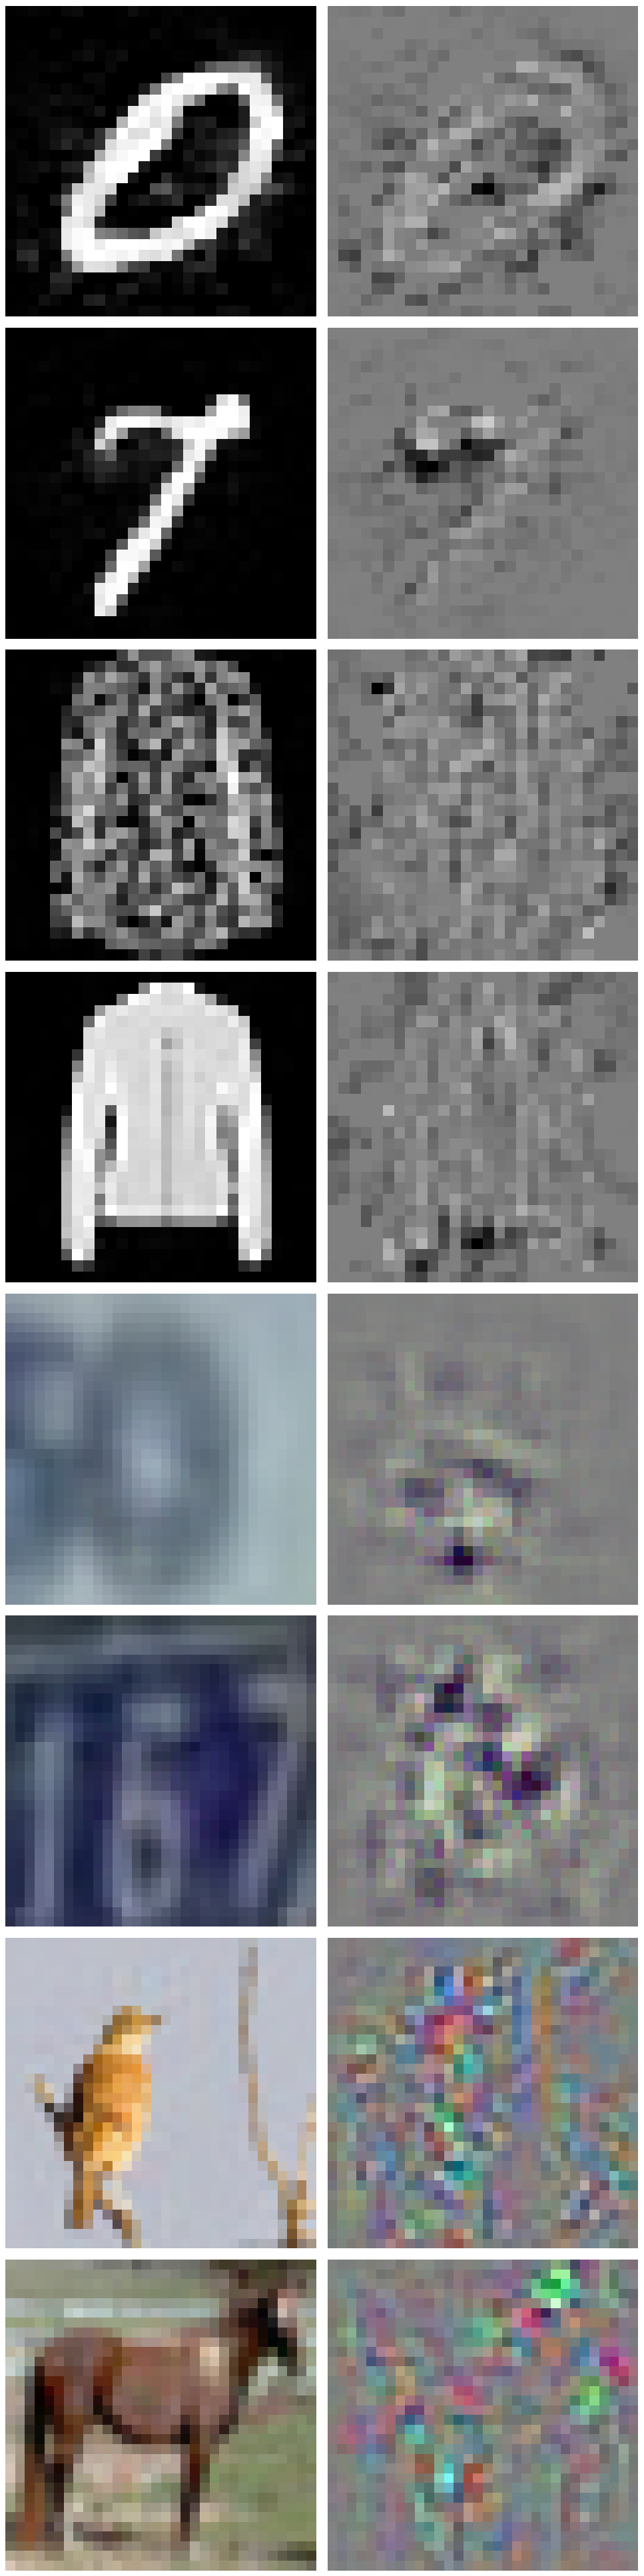
\includegraphics[width=.95\textwidth, right]{deepfool_conv_appendix.pdf}%
		\caption{ConvNet}
	\end{subfigure}
	\caption[DeepFool Adversarial Examples]{DeepFool adversarial examples and perturbations. Pixel values of perturbation images are scaled for visibility}
	\label{fig:deepfool-img}
	
\end{figure}

\begin{figure}
	\centering
	
	\begin{subfigure}{.23\textwidth}
		\centering
		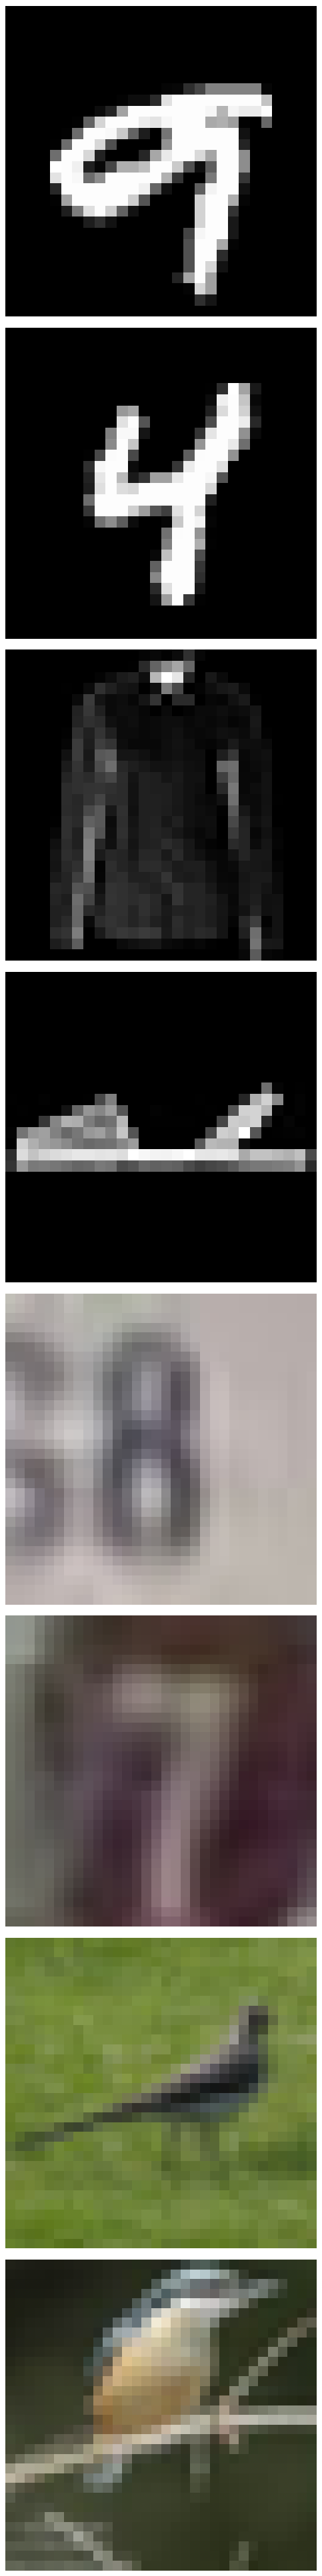
\includegraphics[width=.743478\textwidth, left]{boundary_attack_orig_appendix.pdf}%
		\caption{Original}%
	\end{subfigure}%
	\begin{subfigure}{.36\textwidth}
		\centering
		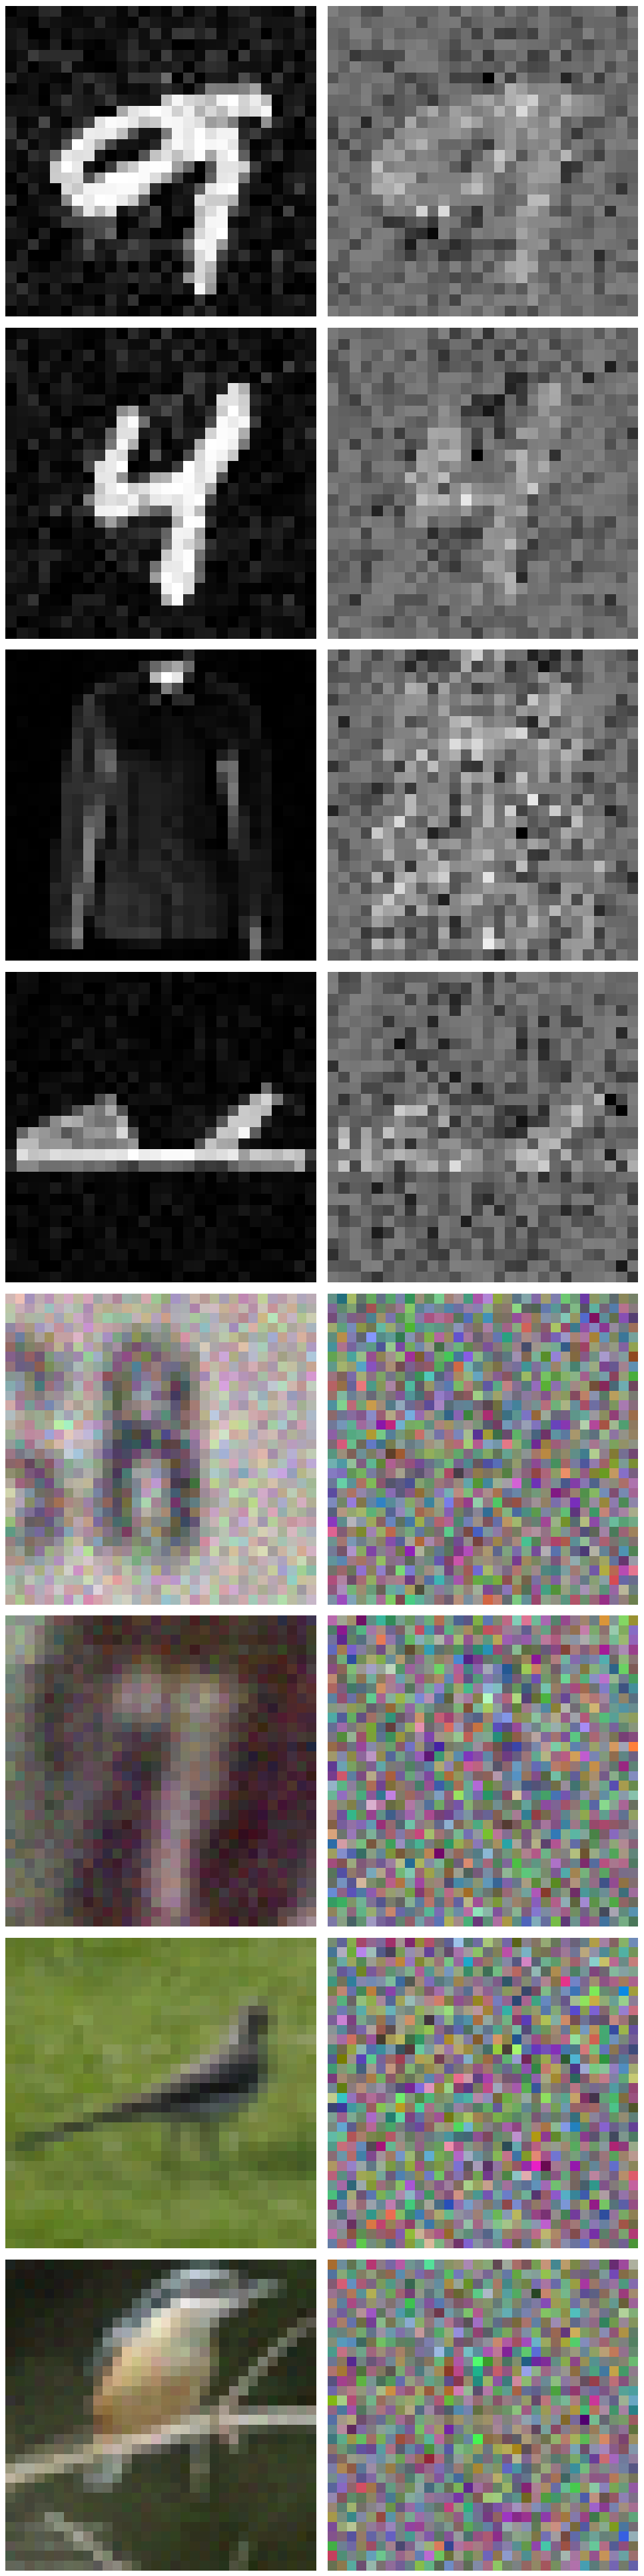
\includegraphics[width=.95\textwidth, center]{boundary_attack_caps_appendix.pdf}%
		\caption{CapsNet}
	\end{subfigure}%
	\begin{subfigure}{.36\textwidth}
		\centering
		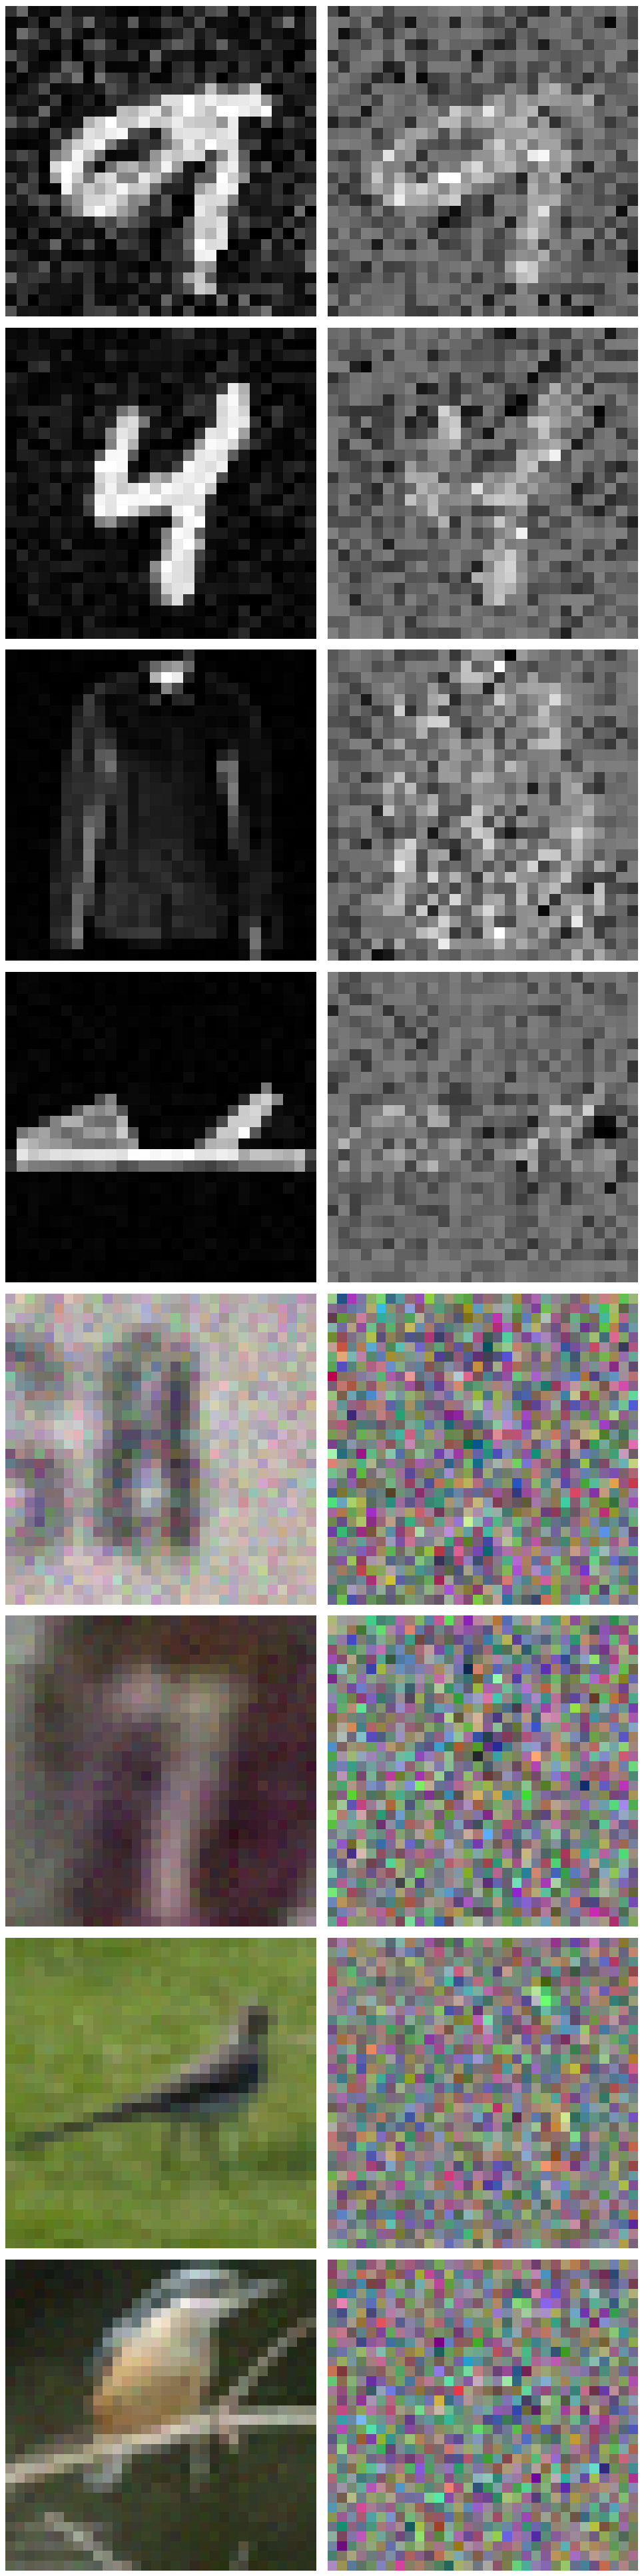
\includegraphics[width=.95\textwidth, right]{boundary_attack_conv_appendix.pdf}%
		\caption{ConvNet}
	\end{subfigure}
	\caption[Boundary Attack Adversarial Examples]{Boundary Attack adversarial examples and perturbations. Pixel values of perturbation images are scaled for visibility}
	\label{fig:boundary-img}
	
\end{figure}

\begin{figure}
	\centering
	
	\begin{subfigure}{.23\textwidth}
		\centering
		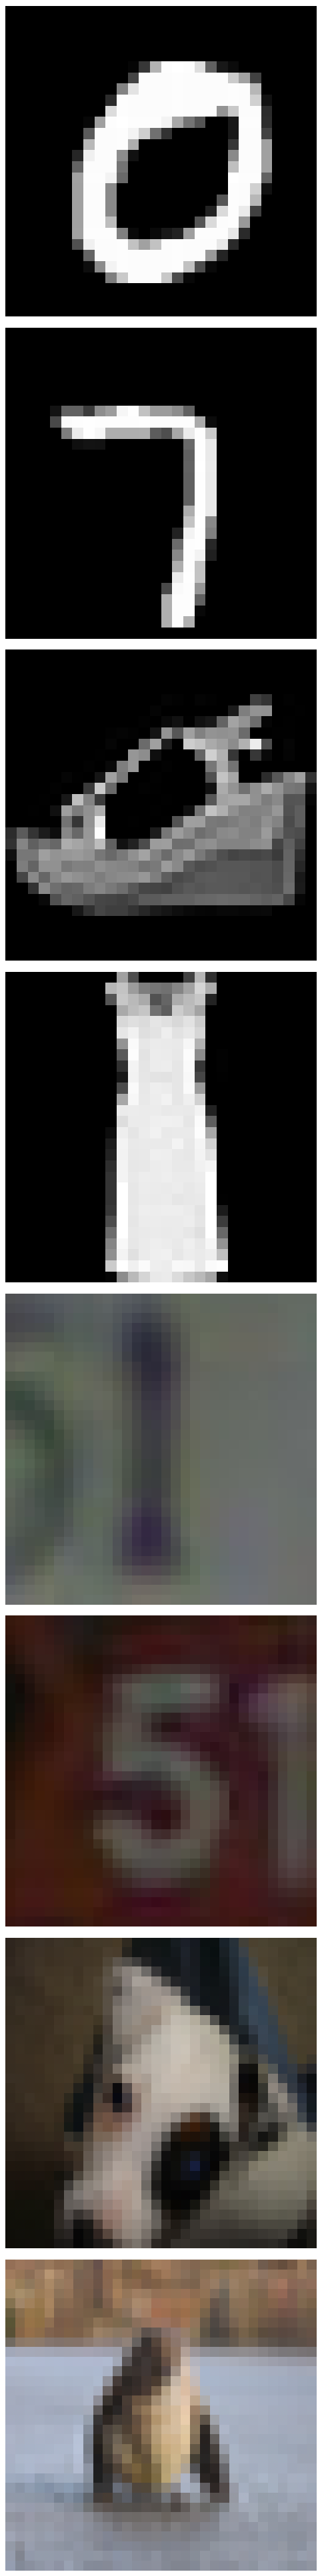
\includegraphics[width=.743478\textwidth, left]{universal_perturbation_orig_appendix.pdf}%
		\caption{Original}%
	\end{subfigure}%
	\begin{subfigure}{.36\textwidth}
		\centering
		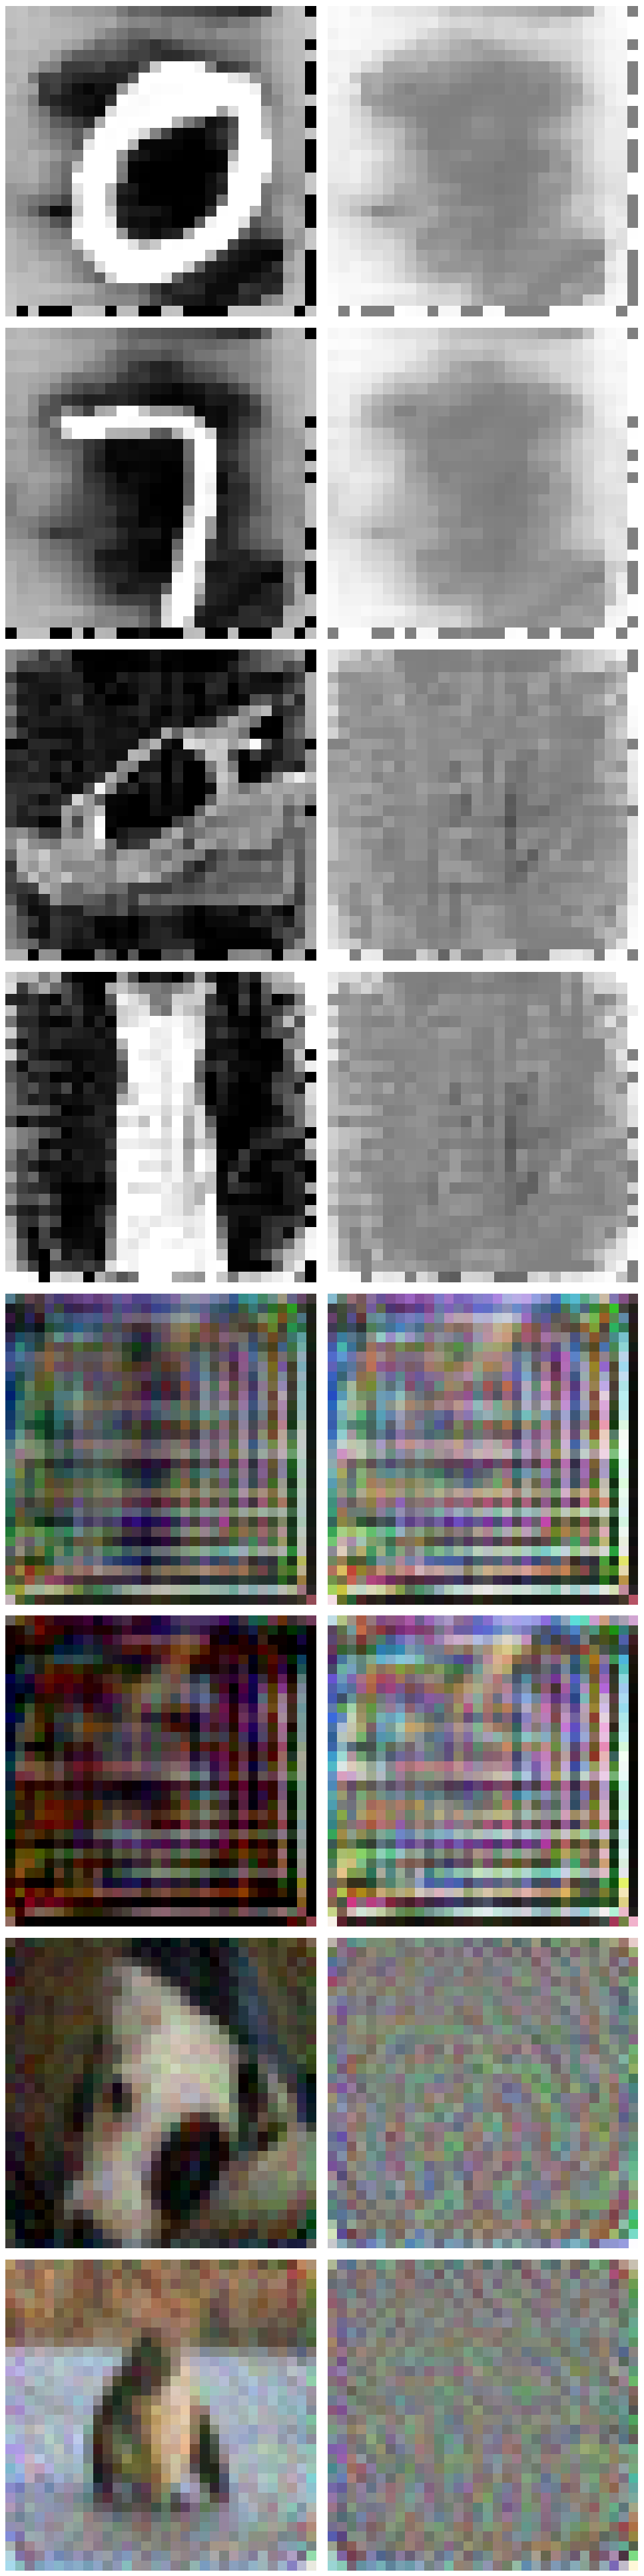
\includegraphics[width=.95\textwidth, center]{universal_perturbation_caps_appendix.pdf}%
		\caption{CapsNet}
	\end{subfigure}%
	\begin{subfigure}{.36\textwidth}
		\centering
		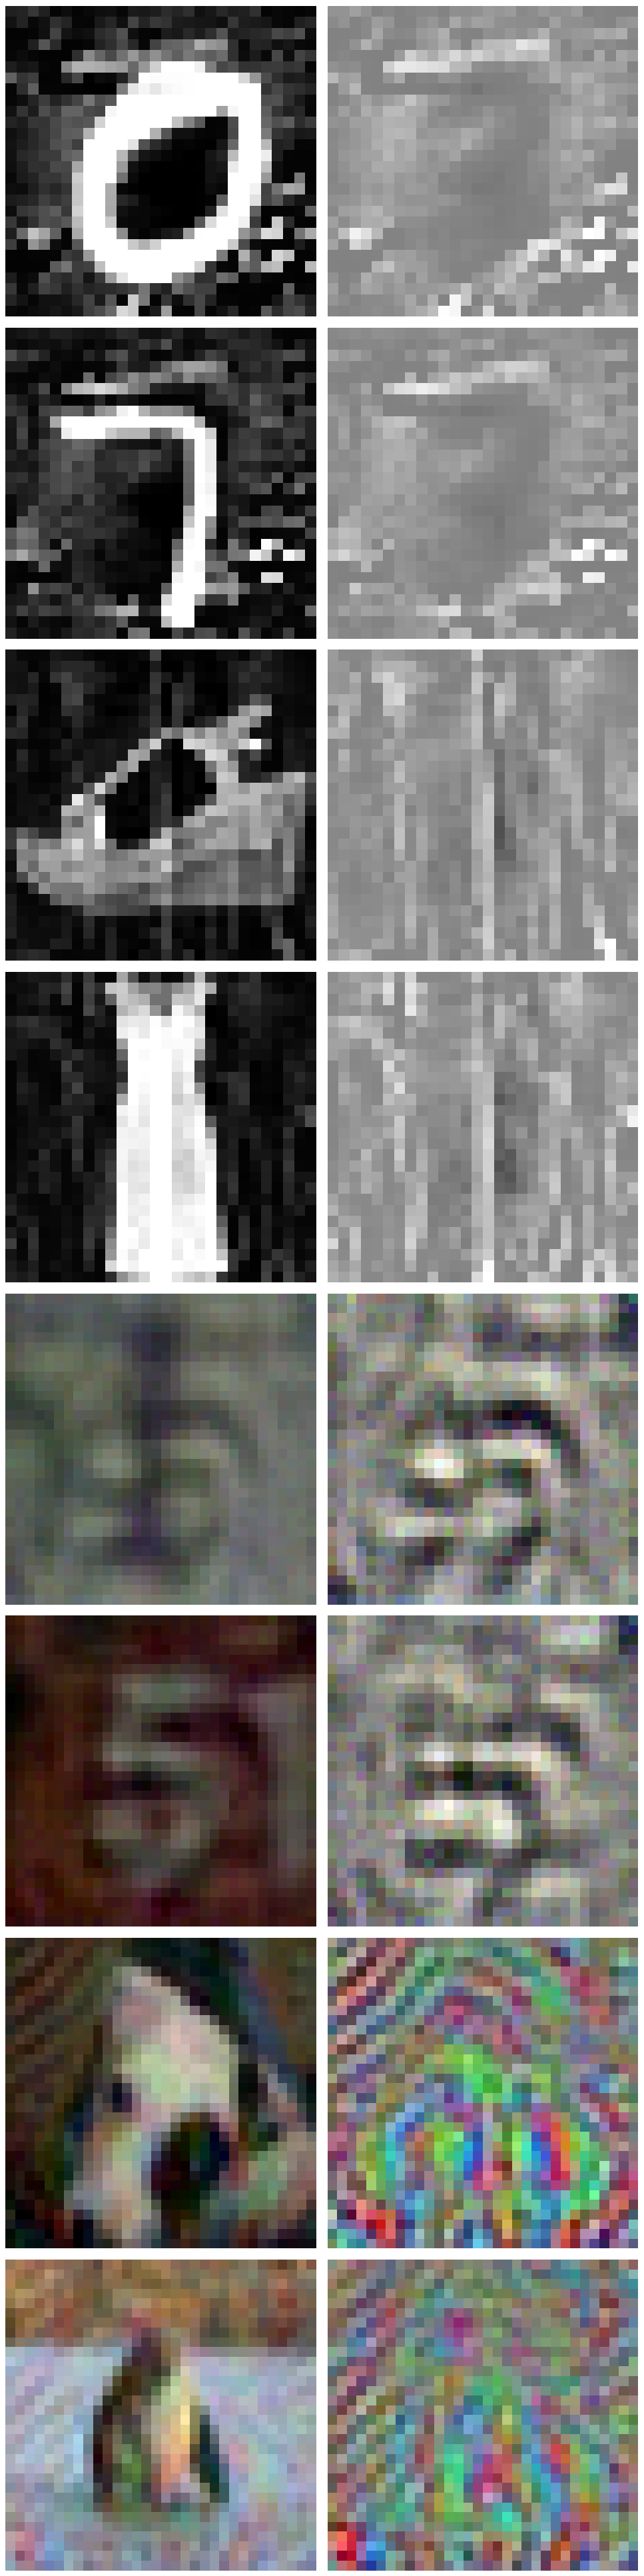
\includegraphics[width=.95\textwidth, right]{universal_perturbation_conv_appendix.pdf}%
		\caption{ConvNet}
	\end{subfigure}
	\caption[Universal Adversarial Perturbation Adversarial Examples]{Universal Adversarial Perturbation adversarial examples and perturbations. Pixel values of perturbation images are scaled for visibility}
	\label{fig:universal-img}
	
\end{figure}
